\chapter{評価}
\label{chap:ledoxea}
本章では開発したスマートフォンアプリDreamTravelerの実験方法(調査対象・観察方法)と実験結果について説明する。

\section{予備実験1:音が夢に与えた回数}
 寝る前の10分間とREM睡眠中に音楽を流すことで、夢に影響を与えるか否かを明らかにするために予備実験に取り組んだ。またスマートフォンは充電をした状態で枕の横に置いてもらうことで、音が脳に届く状態にした。また睡眠を始める前に、海の夢が見たいと被験者に念じてもらった。\\
 20代後半女性の被験者A、40代後半女性の被験者Bと、20代前半女性の被験者Cに何も音楽を流さない場合と流した場合の結果の違いを分析した。海の音を聞く日と効かない日を交互に14日間続けた。そうすることで、音が夢に影響を与えるのか否かの分析を行った。14日間の実験を行ったのは、睡眠に関する実験は体調、その日の活動内容や、被験者の心境によって左右され、データーが変動しやすいためである。図\ref{schedule0}が実験スケジュールと実験結果である。青のハイライトがある日が夢を見た日だ。\\
 夢の具体的な内容について実験後インタビューをした。すると3日間夢を見たと答えた被験者Aは、音のインプットが無い日は会社で働いている夢を見ることが多く、音を流しながら寝た日は10日ほど前に行った沖縄旅行での夢を見たと答えた。一度も海に関連した夢を見なかった被験者Bは、海の音で起こされたりしたため、音は流れていたが全く関係の無い夢を見たと答えた。被験者Cは実験の最後の方で1年前に旅行したアメリカ西海岸に関する夢を見たと答えた。\\
 結果に個人差が見られたが音が無い場合に被験者が海の夢を見たのは1回なのに対し、海の音を流して海の音をmitanoha4回であった。この結果は音が夢にある程度の影響を持っていることを示唆する。また音の影響によってユーザーが起きてしまう事態が発生することが分かった。

\begin{figure}[htbp]
\begin{center}
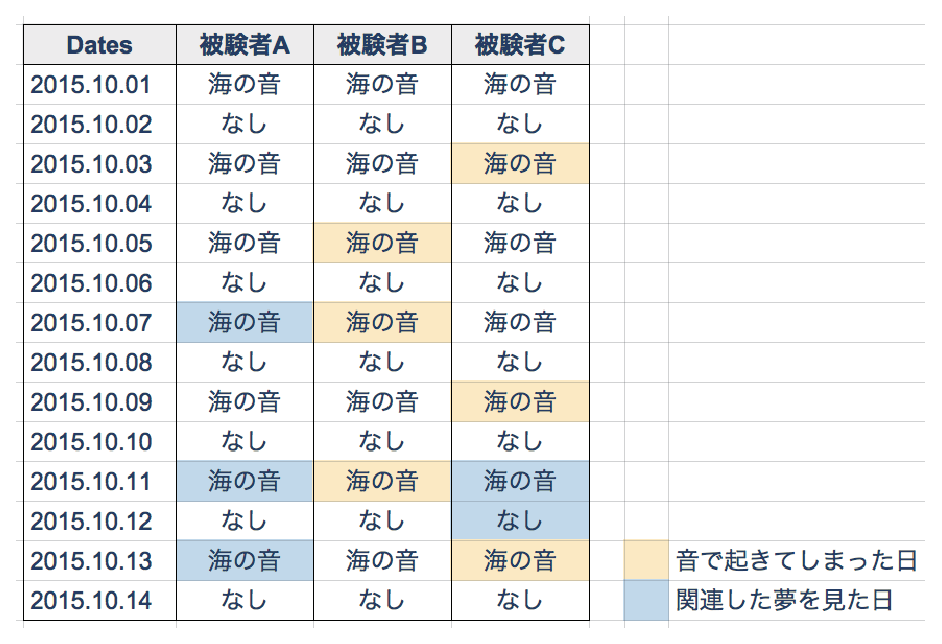
\includegraphics[width=13cm]{eps/schedule0.eps}
\caption{予備実験1:実験スケジュールと実験結果}
\label{schedule}
\end{center}
\end{figure}

\section{予備実験2:睡眠中に流す音の種類とそれが与える影響}
 どのような音がDreamTravelerで使用するのに適しているのかを調べるために予備実験を行った。遠距離恋愛中の交際相手とデートをしている夢を見たいと望む被験者Cに、「音声」「曲」と「自然音」の3種類の音を試した。被験者Cの場合は「音声」は交際相手が被験者Cの名前を語りかけ、思い出のデートの内容について話している声。「曲」は交際相手が被験者Cのために作曲と演奏した曲。「自然音」はアメリカ西海岸の海で交際相手と共に聞いた波の音。図\ref{schedule1}が実験スケジュールと実験結果である。
 夢の具体的な内容について、実験後インタビューをした。関連する夢を見たのは「曲」と「自然音」のときである。11月9日は日本で再開する夢をみて、11月13日は江ノ島で友人と遊ぶ夢をみた。11月15日は交際相手から手紙が届く夢を見た。\\
 実験の結果から、語りかけ口調の音声は被験者を起こしてしまう確率が非常に高いことが示唆される。比べて波の音などの自然音や音楽は比較的被験者を起こす確率が低い。被験者の希望であった遠距離恋愛中の交際相手とデートしたいという要望を実現させることができたのは「曲」であった。

\begin{figure}[htbp]
\begin{center}
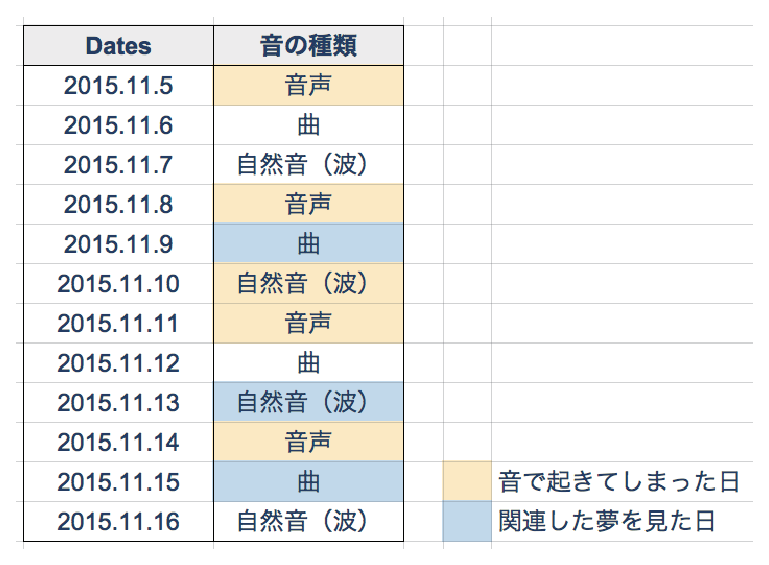
\includegraphics[width=13cm]{eps/schedule1.eps}
\caption{予備実験2:実験スケジュールと実験結果}
\label{schedule}
\end{center}
\end{figure}

\section{実験:音を流すタイミングが夢に与える影響}
 音を流すタイミングによって、夢の結果が変わるのかについて調べるために7人の被験者に15日間の実験に参加してもらった。

\subsection{実験方法}
 被験者にはThe MILD Techniqueに基づいて夢を記憶できる体質になってもらうために実験を開始する5〜10日間前から、被験者には夢日記を書いてもらった。加えて、寝る前に音楽を聴きながら思い出に関する画像を2分間眺めること、思い出について考えならが寝る意識をしてもらった。また6時間以上睡眠を取れる日にのみ実験に臨んでもらった。詳しい事件内容は以下に述べる。実験は1日目は音楽なし、2日目はREM睡眠中音楽あり、3日目は起きる直前のREM睡眠中音楽ありというを繰り返し5回、合計15日間続けてもらった。

\subsection{被験者の詳細}
20歳〜50歳の男女、明晰夢に興味がある7人に参加してもらった。DreamTravelerは日本人のみならず、全世界のユーザーを対象として制作しているので、国籍と性別共に多様性のある被験者を選んだ。また比較的安定したの睡眠活動をしている人を対象にした。下記に具体的な被験者の情報と使用する音を提示する。

被験者1:
\begin{itemize}
\item 国籍:インドネシア人
\item 性別:男性
\item 年齢:30代後半
\item 明晰夢の経験:5回ほど経験している
\item 夢日記を行ったか否か:5日間行った
\item 思い出に由来する音楽:被験者1は音楽にあまり関心がなく、特に思い出に残る音・音楽がなかった。そこで被験者1には日常生活の中で音の刷り込みをした。具体的には、実験10日間前から毎日コーヒーを飲むときにEdith Piafによる"Non je ne regrette rien"という曲。この音楽は映画inceptionの中で夢から覚めるために主人公たちが聴く音楽としても知られている。

\end{itemize}

被験者2:
\begin{itemize}
\item 国籍:日本人
\item 性別:女性
\item 年齢:40代後半
\item 明晰夢の経験:経験したことなし
\item 夢日記を行ったか否か:10日間行った
\item 思い出に由来する音楽:被験者2は30年ほど前の結婚式で流した音楽 The CarpentersによるWe've only just begun
\end{itemize}

被験者3:
\begin{itemize}
\item 国籍:日本人
\item 性別:男性
\item 年齢:50代前半
\item 明晰夢の経験:経験したことなし
\item 夢日記を行ったか否か:10日間行った
\item 思い出に由来する音楽:被験者3は007の映画を体験したいということだった。映画の中で使われているサウンドトラック
\end{itemize}

被験者4:
\begin{itemize}
\item 国籍:アメリカ人
\item 性別:男性
\item 年齢:20代前半
\item 明晰夢の経験:5回以上経験したことがある
\item 夢日記を行ったか否か:5日間行った
\item 思い出に由来する音楽:被験者4は宮崎駿の映画である「魔女の宅急便キキ」を体験したいということだった。映画の中で使われているサウンドトラック
\end{itemize}

被験者5:
\begin{itemize}
\item 国籍:日本人
\item 性別:女性
\item 年齢:20代後半
\item 明晰夢の経験:経験したことない
\item 夢日記を行ったか否か:5日間行った
\item 思い出に由来する音楽:被験者5は今年の9月に社会人ダンス部でダンスを披露したときに利用したCell Block Tangoという曲
\end{itemize}

被験者6:
\begin{itemize}
\item 国籍:アメリカ人
\item 性別:男性
\item 年齢:20代前半
\item 明晰夢の経験:何度か経験したことがある
\item 夢日記を行ったか否か:5日間行った
\item 思い出に由来する音楽:高校時代に演奏したバンドの曲、Fountains of WayneによるStacy's Momという曲
\end{itemize}

被験者7:
\begin{itemize}
\item 国籍:アメリカ人
\item 性別:男性
\item 年齢:20代後半
\item 明晰夢の経験:5回以上経験したことある
\item 夢日記を行ったか否か:5日間ほど行った
\item 思い出に由来する音楽:交際相手のために作曲・演奏した曲Love From The Other Side Of The World\end{itemize}

\subsection{実験結果}
図\ref{schedule}これが実験のスケジュールと実験結果で、図\ref{result}は音楽を流したタイミング別に結果を表した実験結果である。実験の結果から全ての被験者の実験結果を合計し、タイミング別に関連した夢を見たときの確率を導き出した。音を流さないときは1/35、REM睡眠中ずっと音を流したときは10/35、そしてREM睡眠中に夢を見たときは13/35の確率で関連する夢を見た。加えて睡眠中に音楽を流すことで3人の被験者が途中で起きてしまい、睡眠を害してしまった。//
\begin{figure}[htbp]
\begin{center}
\includegraphics[width=15cm]{eps/schedule2.eps}
\caption{実験スケジュールと実験結果}
\label{schedule}
\end{center}
\end{figure}

\begin{figure}[htbp]
\begin{center}
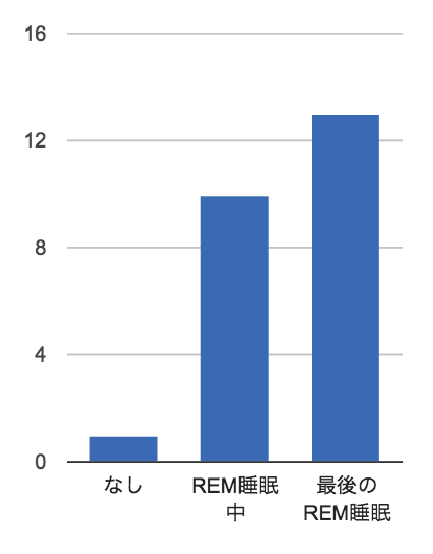
\includegraphics[width=6cm]{eps/result.eps}
\caption{関連した夢を見た回数をタイミング別に表した}
\label{result}
\end{center}
\end{figure}

\section{考察}
 音は夢に影響を与えるのか?
 夢で仮想現実は体験できるのか?
 
予備実験1から被験者の記憶
REMと最後のREMあんまり差がなかったから、起きるの防止のために最後のREMに流すのでOK。刷り込みされた記憶はあえて生活の特定の行動をする時に音楽を聞くことで、体験と関連付けること。例えばある場所で旅行をしている時にずっと聞くことを習慣づけたり、コーヒーを飲む時に必ず聞くと習慣付けるなど。次に、思い出の場所で流れていた音楽。直接的な記憶は自身が深く関わり、繰り返し聞いた音。例えば自ら作曲した歌、演奏した曲、ダンスをした曲)。一方間接的な体験は見た映画やよく聞いていた音楽。

\begin{itemize}
\item 生活の中で音の刷り込みを行った場合(被験者1)\\
 こうすることで記憶と特定の音を紐付けることを試みた。コーヒーを飲むときに決まって聴く曲

\item 思い出を連想させる音楽(被験者2)\\
 するとREM睡眠時に常に音楽を鳴らした3日目と起きる直前のREM睡眠時に音楽を鳴らした5日目に結婚式当初の夢を見ることに成功した。結婚式で流れた曲

\item 間接的な記憶の場合(被験者3・4)\\
 被験者3はインプットしない日の5日目、REM睡眠時に常に音を鳴らした日の5日目、起きる直前のREM睡眠のの5日目にそれぞれ一回ずつ007の夢を見た。すべて実験終盤の結果である。\\被験者4はインプットしない日は全く夢を見なかったことに対して、REM睡眠時に常に音を鳴らした日は2/5の確率で夢を見た。そして起きる直前のREM睡眠時は3/5の確率で夢を見た。

\item 直接的な記憶である場合(被験者5・6・7)\\
 被験者5はインプットを全くしない日は関連した夢を見なかったのに対して、REM睡眠時に常に音を鳴らしたときに1/5の確率でダンスの夢を、起きる直前のREM睡眠のときのみ音を流したときは1/5の確率で関連する夢を見た。\\
 被験者6はインプットを全くしない日は関連した夢を見なかったのに対して、REM睡眠時に常に音を鳴らしたときに1/5の確率でバンド時代の夢を、起きる直前のREM睡眠のときのみ音を流したときは2/5の確率で関連する夢を見た。\\
 被験者6はインプットを全くしない日は関連した夢を見なかったのに対して、REM睡眠時に常に音を鳴らしたときに3/5の確率でバンド時代の夢を、起きる直前のREM睡眠のときのみ音を流したときは4/5の確率で関連する夢を見た。
\end{itemize}


\begin{itemize}
\item 音の効果、有効的なタイミング:
 インプットを全くしない日に夢を見たのは1/35の確率だったのに対し、REM睡眠時に常に音を鳴らしたときは9/35の確率であった。そして起きる直前のREM睡眠のときのみ音を流したときは13/35であった。これらの結果から音による刺激は夢に対してなんらかの操作がかかっているということが示された。またREM睡眠時に常に音を流すのと起きる直前のREM睡眠のときのみ音を流すのでは、直前のみに音を流す方が高い効果が見れた。
\item Dreamtravelerを長く使用すれば使用するほど効果が高まる
\item 睡眠に入る前に瞑想をする時間、写真を眺める時間を加えた方が高い効果が見込まれる
\item 年齢層が高いほど影響を受けにくい可能性がある
\end{itemize}